\chapter{$^{156}$Gd Results and Discussion}

%\section {Oh HAY! FIGURES BIOTCH!}

\begin{figure}
    \centering
    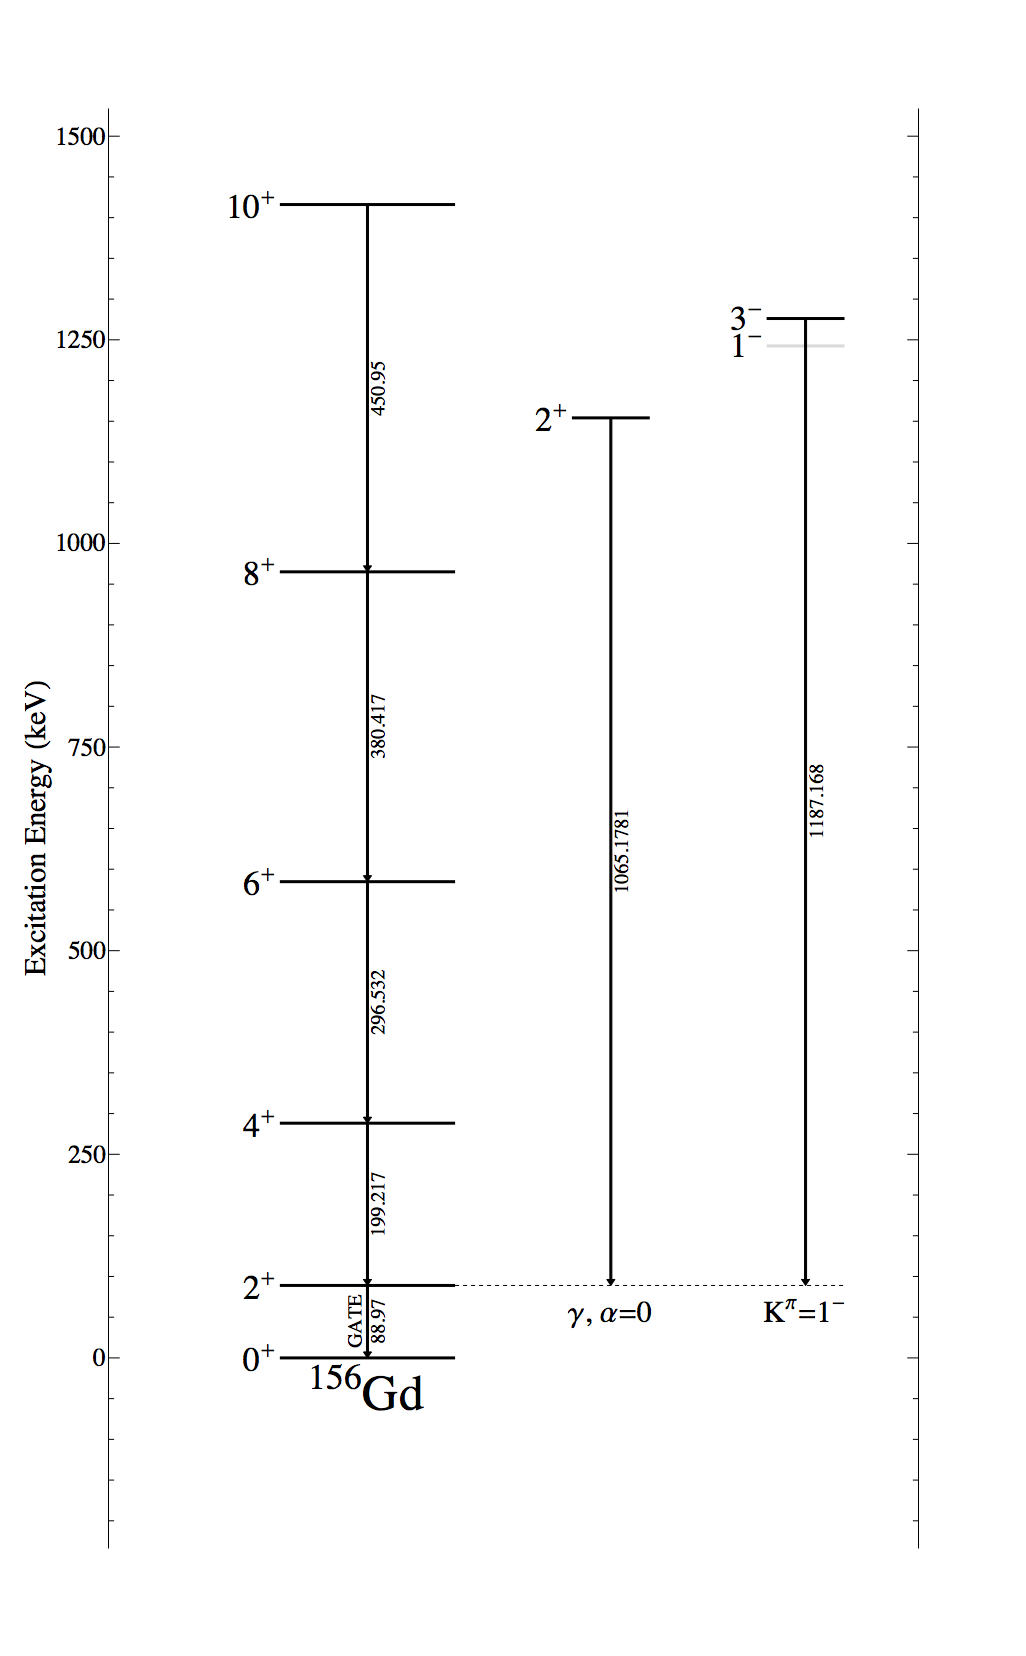
\includegraphics[scale=0.3]{156GdTablesAndFigs/156Gd_2to0.png}
    \caption{Level Scheme of $^{156}$Gd. The gamma ray of the $2^+$\rightarrow$0^+$ transition in the ground state was gated on. It was then compared with the gated spectrum from the gamma ray of the $4^+$\rightarrow$2^+$ transition in the ground state. Peaks only appearing in the first gate were assumed to go into the $2^+$ state, and assignments were made. Due to the low energy of the $2^+$\rightarrow$0^+$ transition, the efficiency was lower, and it is likely that transitions into the $2^+$ state were missed. The levels are organized by band. The lower levels of the band, unseen by gamma rays in this gate, are in gray.}
    \label{fig:156_2to0}
\end{figure}

\begin{figure}
    \centering
    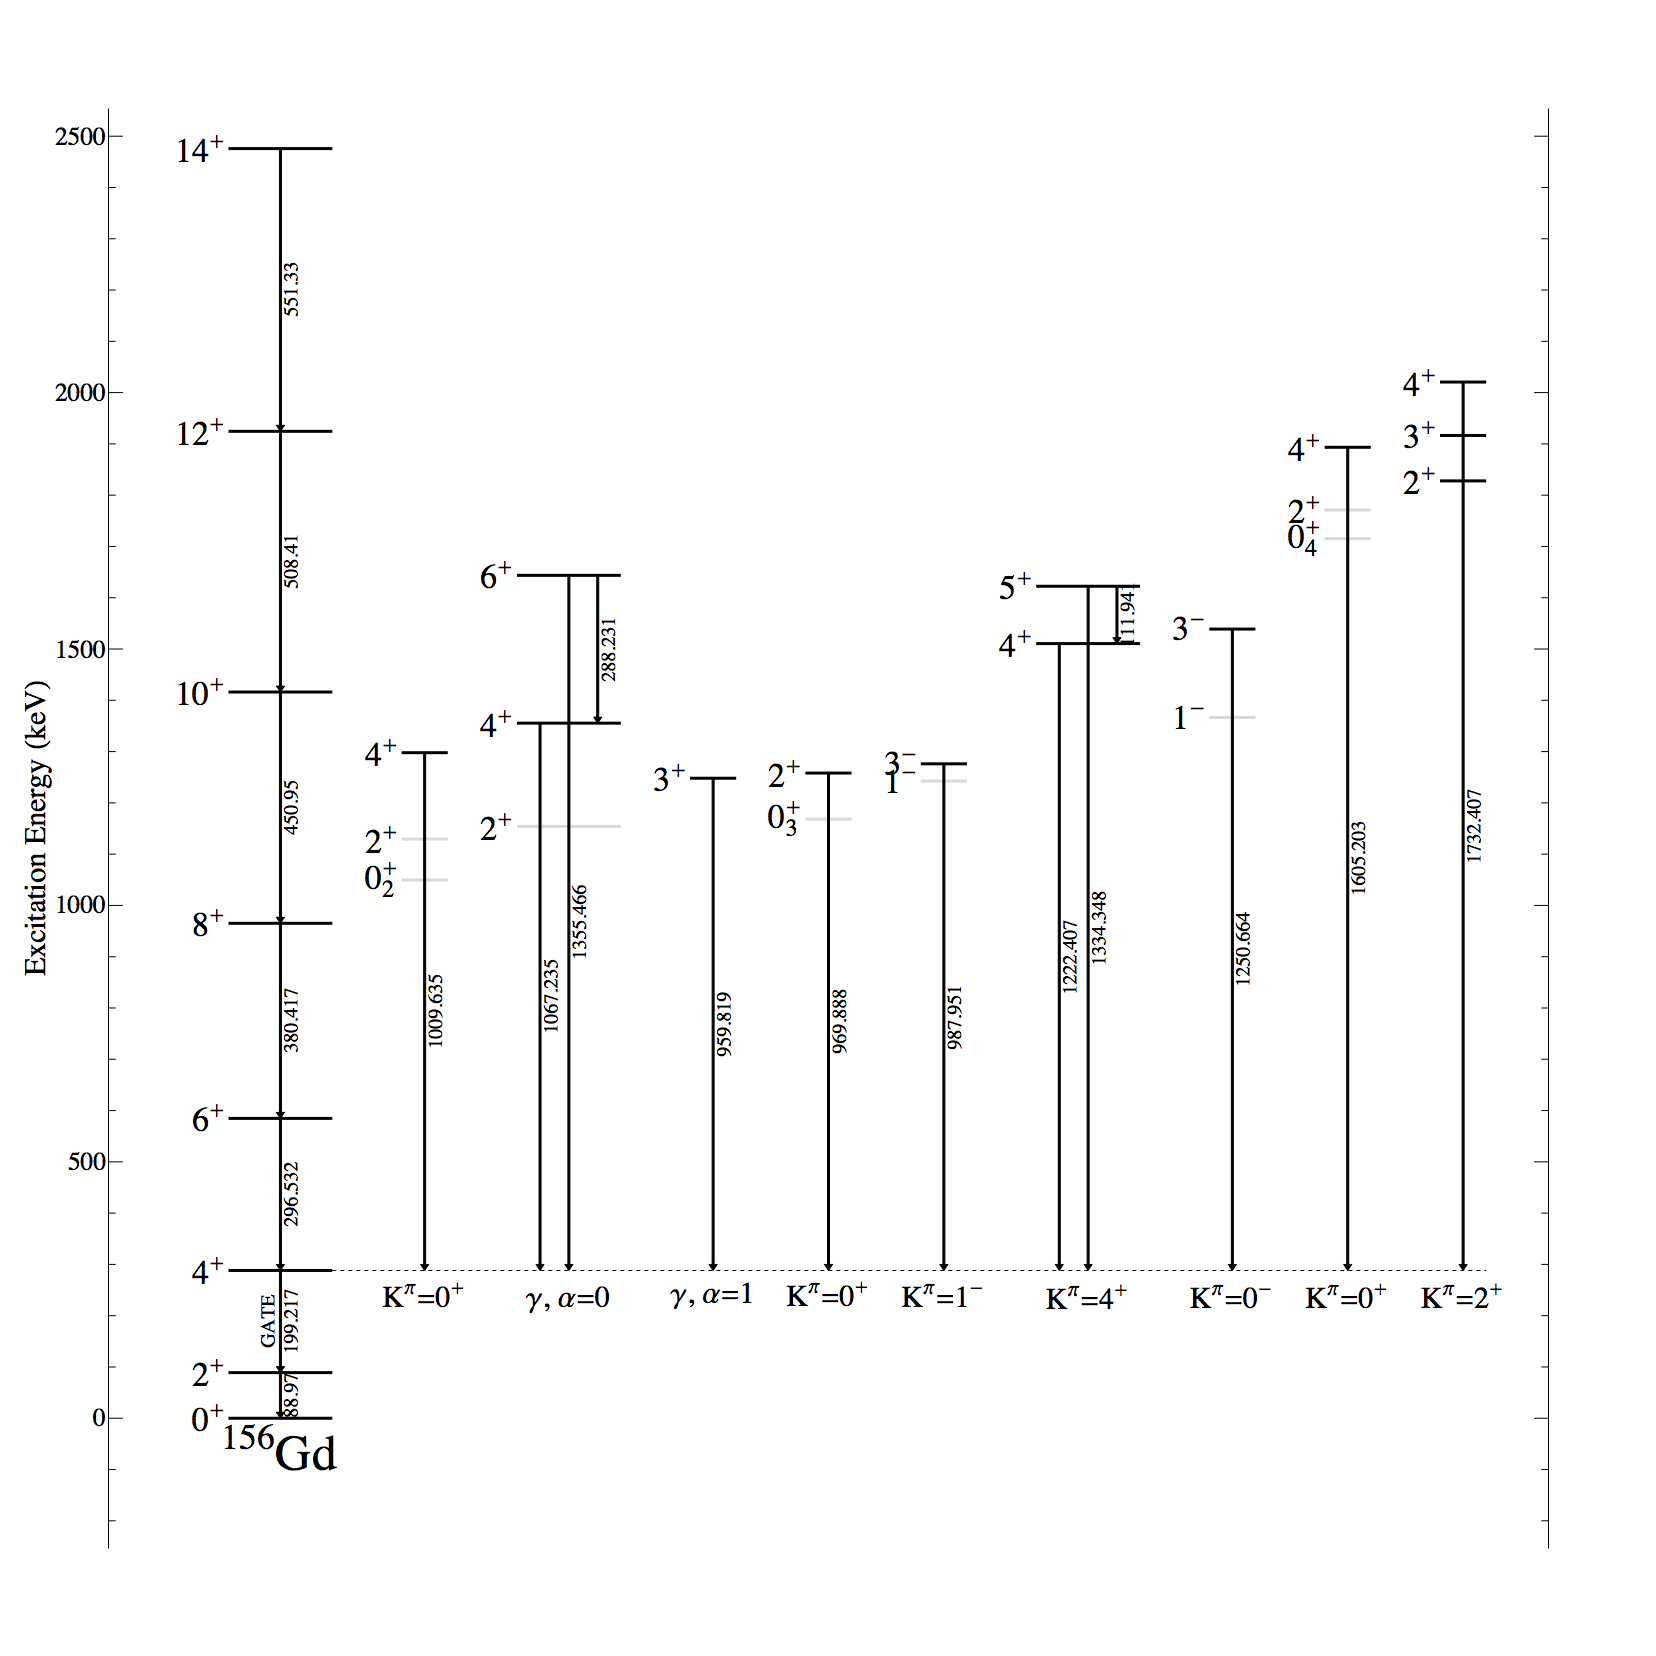
\includegraphics[scale=0.28]{156GdTablesAndFigs/156Gd_4to2.png}
    \caption{Level Scheme of $^{156}$Gd. The gamma ray of the $4^+$\rightarrow$2^+$ transition in the ground state was gated on. It was then compared with the gated spectrum from the gamma ray of the $6^+$\rightarrow$4^+$ transition in the ground state. Peaks only appearing in the first gate were assumed to go into the $4^+$ state, and assignments were made. Additionally, these peaks were also gated on, to look for cascades leading into the $4^+$ state, which were found in several cases. The levels are organized by band. The lower levels of the band, unseen by gamma rays in this gate, are in gray.}
    \label{fig:156_4to2}
\end{figure}

\begin{figure}
    \centering
    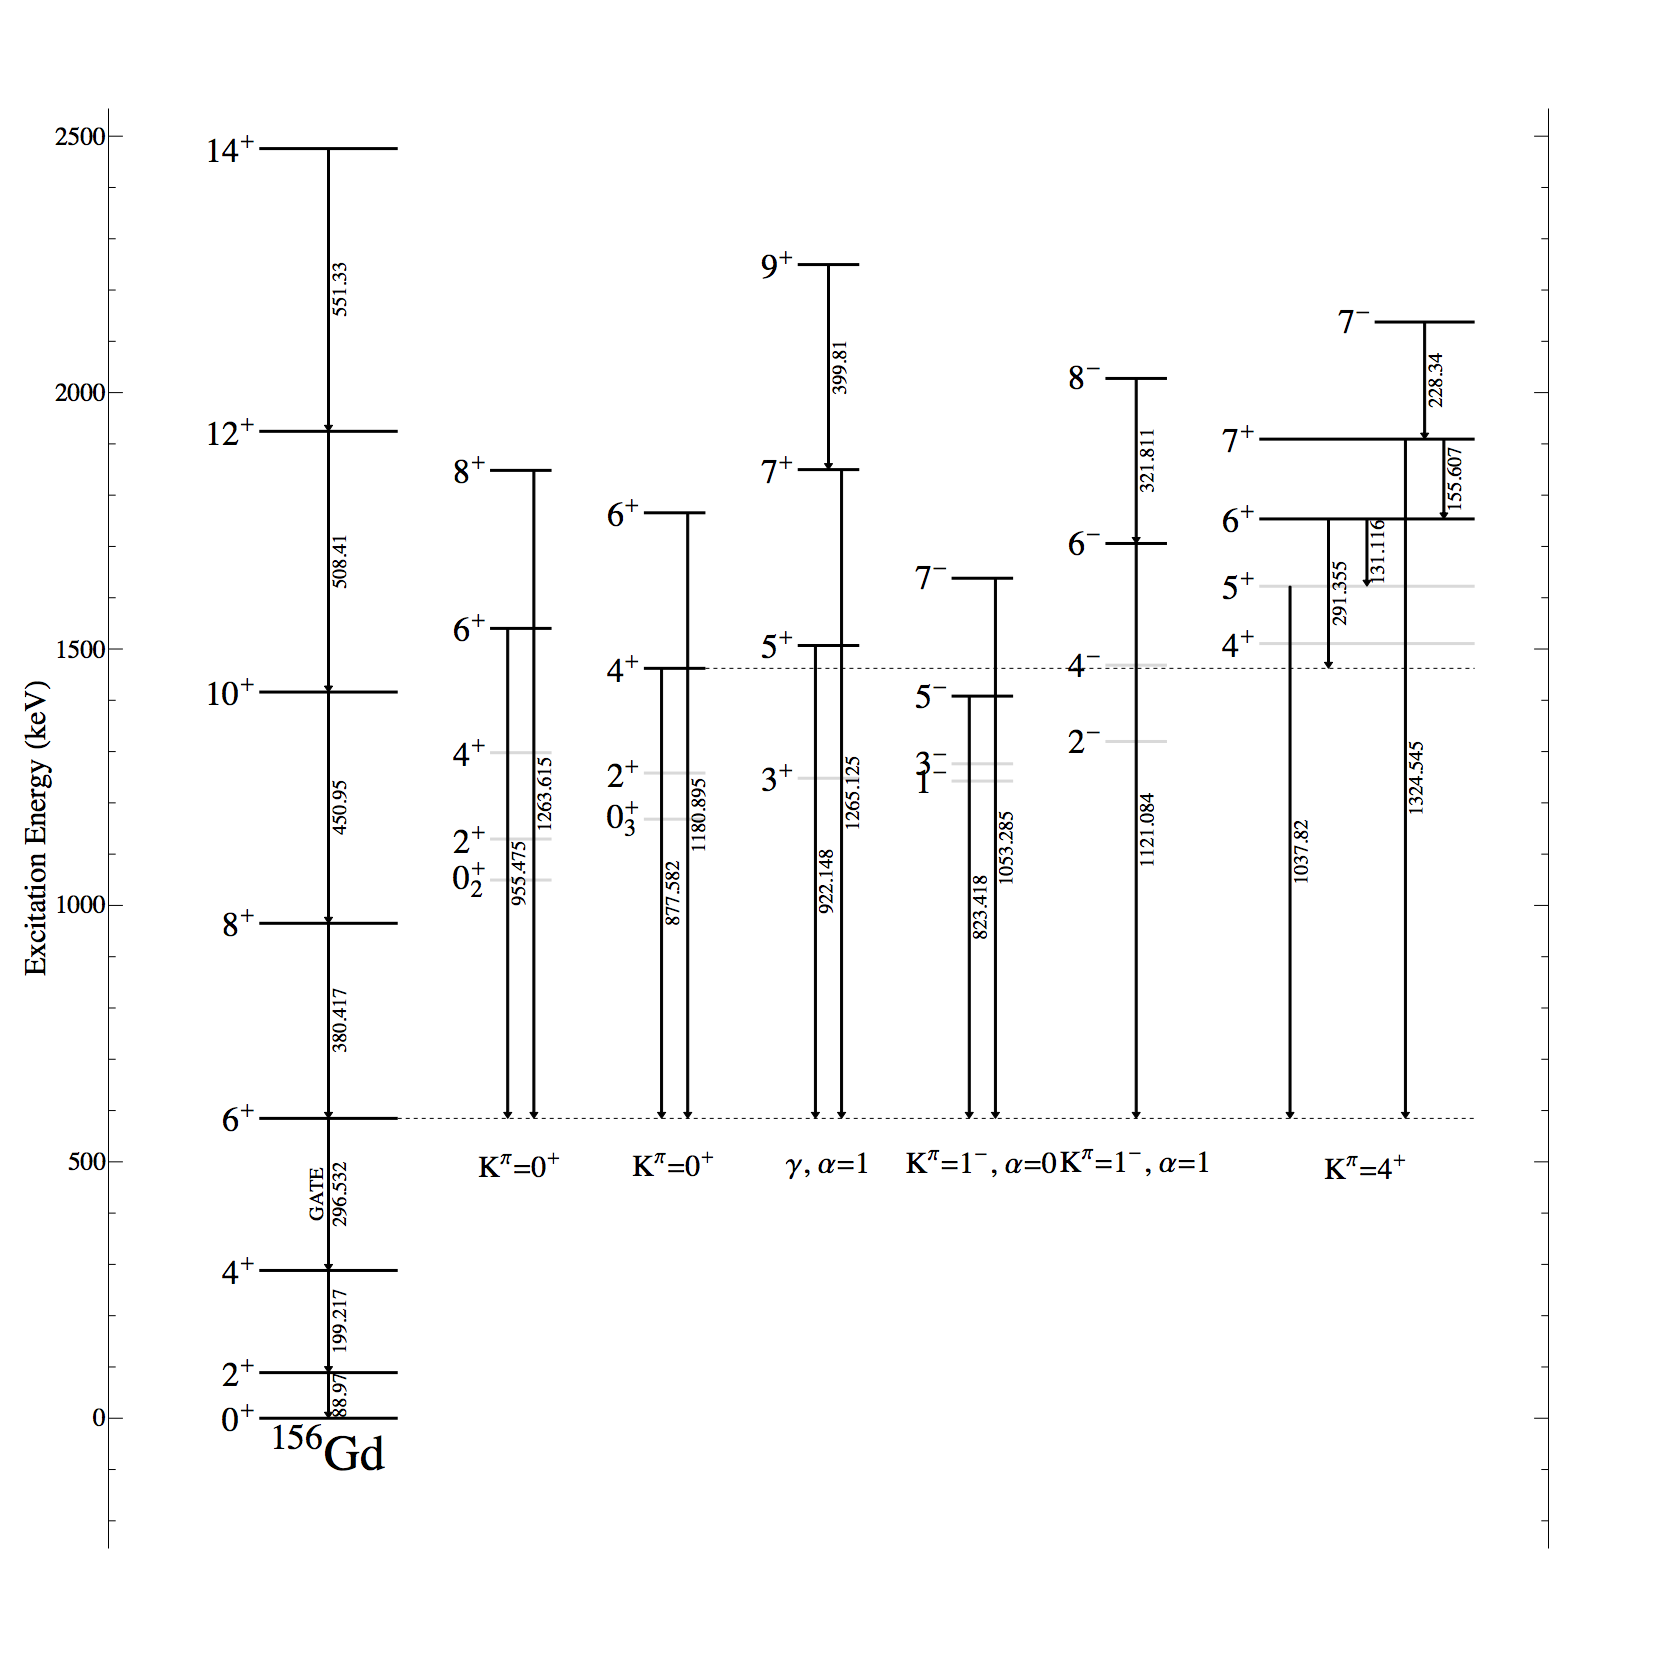
\includegraphics[scale=0.28]{156GdTablesAndFigs/156Gd_6to4.png}
    \caption{Level Scheme of $^{156}$Gd. The gamma ray of the $6^+$\rightarrow$4^+$ transition in the ground state was gated on. It was then compared with the gated spectrum from the gamma ray of the $8^+$\rightarrow$6^+$ transition in the ground state. Peaks only appearing in the first gate were assumed to go into the $6^+$ state, and assignments were made. Additionally, these peaks were also gated on, to look for cascades leading into the $6^+$ state, which were found in several cases. The levels are organized by band. The lower levels of the band, unseen by gamma rays in this gate, are in gray.}
    \label{fig:156_6to4}
\end{figure}

\begin{figure}
    \centering
    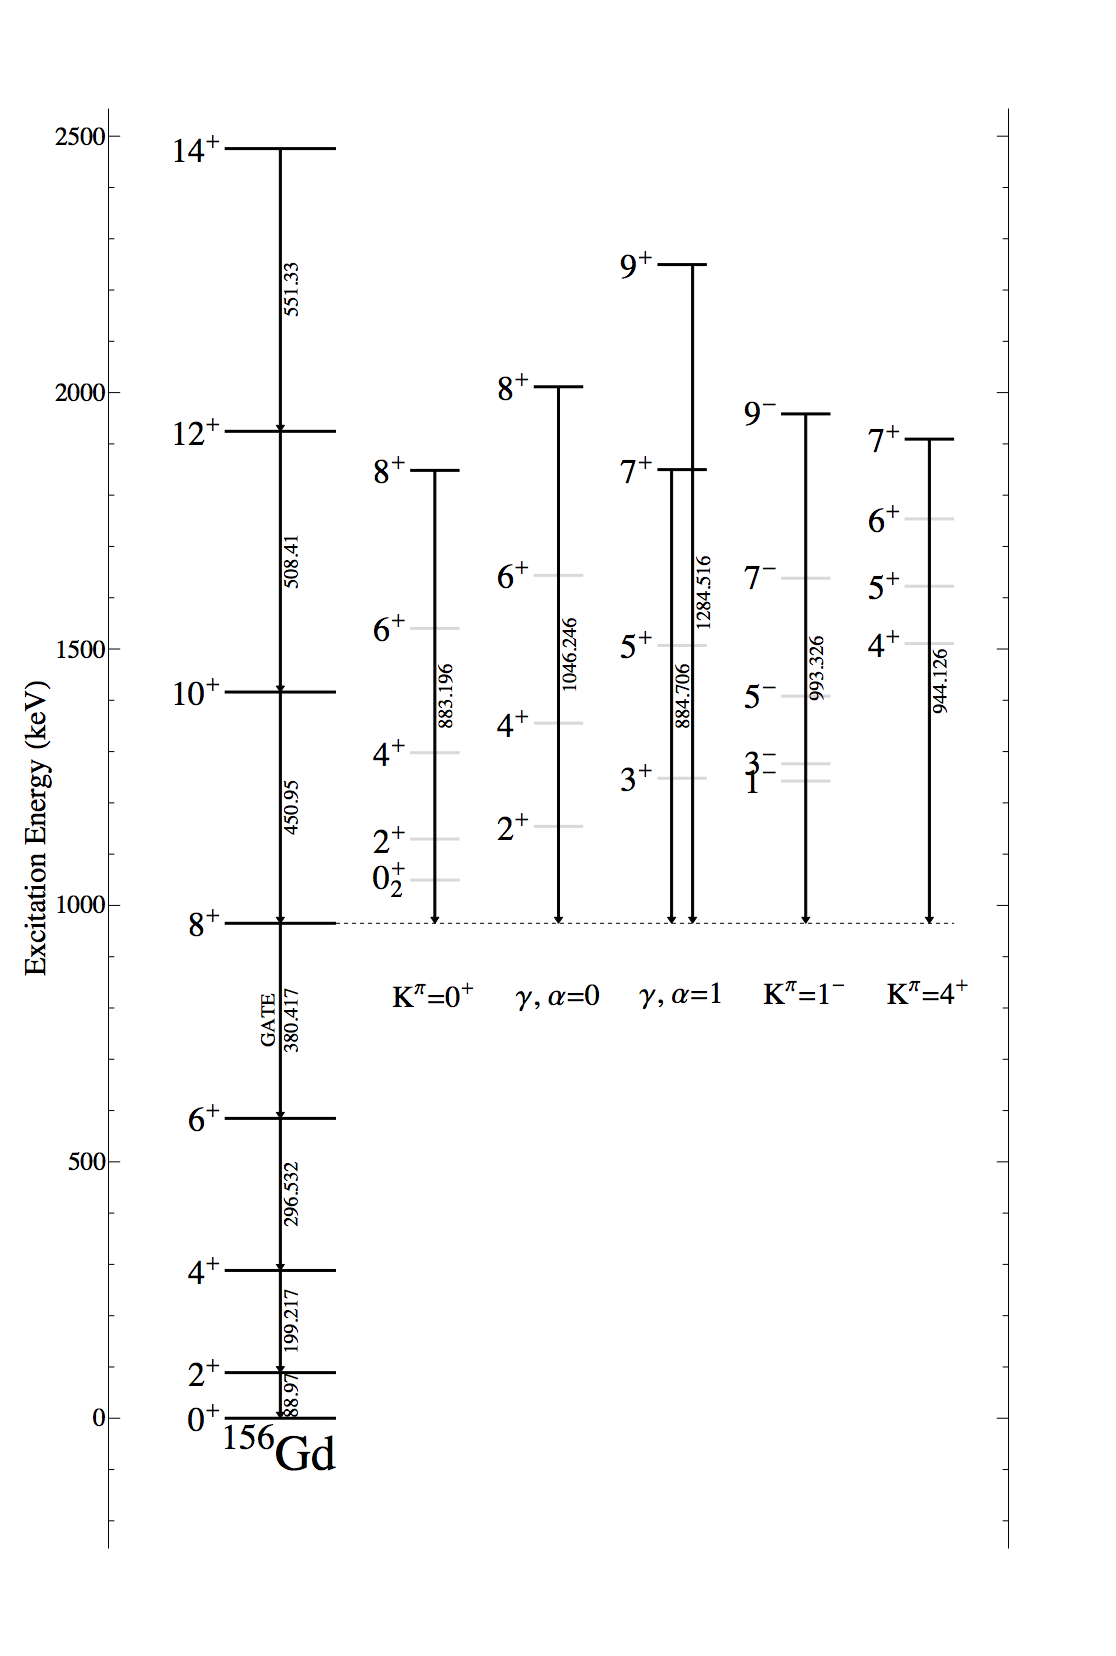
\includegraphics[scale=0.3]{156GdTablesAndFigs/156Gd_8to6.png}
    \caption{Level Scheme of $^{156}$Gd. The gamma ray of the $8^+$\rightarrow$6^+$ transition in the ground state was gated on. It was then compared with the gated spectrum from the gamma ray of the $10^+$\rightarrow$8^+$ transition in the ground state. Peaks only appearing in the first gate were assumed to go into the $8^+$ state, and assignments were made. Additionally, these peaks were also gated on, to look for cascades leading into the $8^+$ state, which were found in several cases. The levels are organized by band. The lower levels of the band, unseen by gamma rays in this gate, are in gray.}
    \label{fig:156_8to6}
\end{figure}

%\section{LOOK! A TABLE!}

\begin{landscape}
\footnotesize
    \begin{longtable}{c|c|c|c|c|c|c|c|c|c}
    \caption{$^{156}$Gd Ground State Band Internal Conversion Coefficients from Singles}
        \label{tab:156Gd_Single_ICC_GS}\\
    \toprule
$E$ (keV)	&	$J^{\pi}	\rightarrow	J^{\pi}$	&	$E_i$ (keV)	&	$E_f$ (keV)	&	$T_{1/2}$ (fs)	&	Multipolarity	&	Shell & $\alpha$ (This Work)	&	$\alpha$  (Th)	&	$\alpha$ (Konijn)	\\
\hline		
\endfirsthead
    \caption[]{$^{156}$Gd Ground State Band Internal Conversion Coefficients from Singles}\\
    \toprule
$E$ (keV)	&	$J^{\pi}	\rightarrow	J^{\pi}$	&	$E_i$ (keV)	&	$E_f$ (keV)	&	$T_{1/2}$ (fs)	&	Multipolarity	&	Shell & $\alpha$ (This Work)	&	$\alpha$  (Th)	&	$\alpha$ (Konijn)	\\
\hline		
\endhead
\endfoot
\multicolumn{10}{p{1.4\textwidth}}{A list of the ground state conversion coefficients from $^{156}$Gd. Multipolarities and mixing ratios were taken from NNDC. Unless otherwise stated, the $\alpha$ values are $\alpha_K$. An angular distribution correction has been applied based on multipolarities for pure transitions, and those with known mixing ratios. The first error is statistical, the second is systematic. Numbers are compared with Konijn et al. \citep{konijn81:_156gd} Starred values in the Konijn data were used as calibration points.}
\endlastfoot
198.58	&	$4^+	\rightarrow	2^+$	&	288.187	&	88.97	&	111900	&	E2	& K &	0.1667 (4)$^{+46}_{-45}$	&	0.1565 (22)	&	0.199 (36)	\\
	&				&		&		&		&		& L &	0.0537 (1)$^{+16}_{-15}$	&	0.0531 (8)	&		\\
	&			&		&		&		&		& M &	0.0170 (1) (5)	&	0.0122 (2)	&		\\ \hline
296.04	&	$6^+	\rightarrow	4^+$	&	584.715	&	288.187	&	15800	&	E2 & K	&	0.0572 (1) (18)	&	0.0477 (7)	&	0.04683*	\\
	&				&		&		&		&	& L	&	0.0121 (1) (4)	&	0.0115 (2)	&		\\
	&				&		&		&		&	& M	&	0.0036 (1) (1) &	0.0026 (1)	&		\\ \hline
379.92	&	$8^+	\rightarrow	6^+$	&	965.134	&	584.715	&	4320	&	E2 & K	&		0.0274 (1) (9)	&	0.0235 (4)	&	0.038 (10)	\\
	&				&		&		&		&	& L	&	0.0050 (1) (2)	&	0.0048 (1)	&		\\
	&				&		&		&		&	& M	&	0.0013 (1) (1)	&	0.0011 (1)	&		\\ \hline
450.64	&	$10^+	\rightarrow	8^+$	&	1416.078	&	965.134	&	1900	&	E2	& K &	0.0152 (2) (5)	&	0.01483 (21)	& 0.0145*		\\
	&				&		&		&		&	& L	&	0.0028 (1) (1)	&	0.00279 (4)	&		\\
	&				&		&		&		&	& M	&	0.0010 (1) (1)	&	0.000621 (9)	&		\\ 
\bottomrule
    \end{longtable}
\end{landscape}

\begin{landscape}
    \begin{longtable}{>{\footnotesize}c|>{\footnotesize}c|>{\footnotesize}c|>{\footnotesize}c|>{\footnotesize}c|>{\footnotesize}c|>{\footnotesize}c|>{\footnotesize}c|>{\footnotesize}c|>{\footnotesize}c|>{\footnotesize}c}
    \caption{$^{156}$Gd Internal Conversion Coefficients from Singles}
        \label{tab:156Gd_Single_ICC_Corr}\\
    \toprule
$E$ (keV)	&	$J^{\pi}	\rightarrow	J^{\pi}$	&	$E_i$ (keV)	&	$E_f$ (keV)	&	$T_{1/2}$ (fs)	&	Multipolarity	&	$\delta$	& Shell &	$\alpha$ (This Work)	&	$\alpha$  (Theory)\citep{kibedi08:_BRICC}	&	$\alpha$ (Konijn)\citep{konijn81:_156gd}	\\
\hline		
\endfirsthead
    \caption[]{$^{156}$Gd Internal Conversion Coefficients from Singles}\\
    \toprule
$E$ (keV)	&	$J^{\pi}	\rightarrow	J^{\pi}$	&	$E_i$ (keV)	&	$E_f$ (keV)	&	$T_{1/2}$ (fs)	&	Multipolarity	&	$\delta$ & Shell &	$\alpha$ (This Work)	&	$\alpha$  (Theory)\citep{kibedi08:_BRICC}	&	$\alpha$ (Konijn)\citep{konijn81:_156gd}	\\
\hline		
\endhead
\endfoot
\multicolumn{11}{p{1.4\textwidth}}{A list of conversion coefficients from $^{156}$Gd. Multipolarities and mixing ratios were taken from the nuclear date sheets\citep{reich12:_nds_156}. Unless otherwise stated, the $\alpha$ values are $\alpha_K$. An angular distribution correction has been applied based on multipolarities for pure transitions, and those with known mixing ratios. The first error is statistical, the second is systematic. Numbers are compared with Konijn et al\citep{konijn81:_156gd}.}
\endlastfoot
227.90	&	$7^-_{7^-}	\rightarrow 7^+_{4^+}$	&	2137.6	&	1909.26	&	1300000000	&	E1	&	& K	&	0.4687 (50)$^{+85}_{-84}$	&	0.0272 (4)	&	0.063 (13)	\\
	&			&		&		&		&		&	& LM	&	0.1073 (20) (20)	&	0.0049 (6)	&		\\ \hline
321.92	&	$8^-_{1^-}	\rightarrow	6^-_{1^-}$	&	2027.1	&	1705.799	&		&	E2	&		& K &	0.0290 (13) (9)	&	0.0378 (6)	&	0.025 (7)	\\ \hline
355.87	&	$4^+_{4^+}	\rightarrow	2^+_{\gamma}$	&	1510.594	&	1154.152	&	189000	&	E2	&		& K &	0.0158 (6) (5)	&	0.0281 (4)	&	\\ \hline
399.56	&	$9^+_{\gamma}	\rightarrow	7^+_{\gamma}$	&	2249.65	&	1849.84	&		&	E2	&		& K &	0.0077 (8) (3)	&	0.0205 (3)	&	0.026 (5)	\\ \hline
921.83	&	$5^+_{\gamma}	\rightarrow	6^+_{gs}$	&	1506.863	&	584.715	&	400	&	E2	&		& K &	0.0041 (9) (5) &	0.0028 (1)	&	0.0030 (7)	\\ \hline
1040.470	&	$2^+_{0^+_{2}}	\rightarrow	2^+_{gs}$	&	1129.437	&	88.970	&		&	E2+E0+M1	&	$-5.9^{+14}_{-28}$	& K &	0.0152 (10) (2)	&	0.0022 (1)	&	0.014 (3)	\\ \hline
1059.31	&	$6^+_{\gamma}	\rightarrow	6^+_{gs}$	&	1643.653	&	584.715	&		&	E2	&		& K &	0.0013 (5) (1)	&	0.0021 (1)	&	0.0013 (8)	\\ \bottomrule
    \end{longtable}
\end{landscape}

	\begin{ThreePartTable}
		\begin{longtable}{>{\footnotesize}c|>{\footnotesize}c|>{\footnotesize}c|>{\footnotesize}c|>{\footnotesize}c|>{\footnotesize}c|>{\footnotesize}c}
			\caption{Uncorrected $^{156}$Gd Internal Conversion Coefficients from Singles\label{tab:156Gd_Single_ICC_Uncorr} }\\
			\multicolumn{6}{c}{(a)} \\
			\toprule
	& & & & & \\
	$E$ (keV)	&	$J^{\pi}	\rightarrow	J^{\pi}$	&	$E_i$ (keV)	&	$E_f$ (keV)	& $T_{1/2}$ (fs) &	Multipolarity	&	$\delta$ \\
	\hline
	\endfirsthead
	\caption[]{Uncorrected $^{156}$Gd Internal Conversion Coefficients from Singles} \\
	\multicolumn{6}{c}{(a)} \\
	\toprule
	$E$ (keV)	&	$J^{\pi}	\rightarrow	J^{\pi}$	&	$E_i$ (keV)	&	$E_f$ (keV)	& $T_{1/2}$ (fs) &	Multipolarity	&	$\delta$ \\
	\hline
	\endhead
154.94	&	$4^+_{4^+}	\rightarrow	4^+_{\gamma}$	&	1510.594	&	1355.422	&	189000	&	M1+E2	&	0.48	\\
	&	$7^+_{4^+}	\rightarrow	6^+_{4^+}$	&	1909.26	&	1753.653	&		&	(M1+E2)	&	0.29	\\ \hline
883.86	&	$8^+_{0^+_{2}}	\rightarrow	8^+_{gs}$	&	1848.33	&	965.134	&		&	E0+E2	&		\\
	&	$7^+_{\gamma}	\rightarrow	8^+_{gs}$	&	1849.84	&	965.134	&		&	E2(+M1)	&		\\ 
	&		&		&	&		&	\\ \hline
955	&	$6^+_{0^+_{2}}	\rightarrow	6^+_{gs}$	&	1540.19	&	584.715	&		&	E0+E2	&		\\ 
959.88	&	$0^+_{0^+_{2}}	\rightarrow	2^+_{gs}$	&	1049.487	&	88.97	&	1800	&	E2	&			\\
	&	$3^+_{\gamma}	\rightarrow	4^+_{gs}$	&	1248.006	&	288.197	&	580	&	E2+M1	&	-12	\\ \hline
1009.33	&	$4^+_{0^+_{2}}	\rightarrow	4^+_{gs}$	&	1297.822	&	288.197	&	1600	&	E0+E2,M1	&		\\ 
&		&		&	&		&	\\ \hline
1045.48	&	$8^+_{\gamma}	\rightarrow	8^+_{gs}$	&	2011.38	&	965.134	&		&	E2(+M1)	&		\\ 
&		&		&	&		&	\\ 
1052.61	&	$7^-_{1^-}	\rightarrow	6^+_{gs}$	&	1638	&	584.715	&		&	E1	&		\\ \hline
1065.74	&	$2^+_{\gamma}	\rightarrow	2^+_{gs}$	&	1154.152	&	88.97	&	568	&	E2+M1	&	-16	\\
	&	$4^+_{\gamma}	\rightarrow	4^+_{gs}$	&	1355.422	&	288.187	&	540	&	E2+M1	&	-4	\\ \hline
1158.65	&	$2^+_{\gamma}	\rightarrow	0^+_{gs}$	&	1154.152	&	0	&	568	&	E2	&		\\
	&	$3^+_{\gamma}	\rightarrow	2^+_{gs}$	&	1248.006	&	88.97	&	580	&	E2+M1	&	-11.8	\\ \hline
1168.69	&	$0^+_{0^+_{3}}	\rightarrow	0^+_{gs}$	&	1168.186	&	0	&	5000	&	E0	&		\\
	&	$2^+_{0^+_{3}}	\rightarrow	2^+_{gs}$	&	1258.075	&	88.97	&	1540	&	E2+M1+E0	&	0.38	\\ \hline
1222.22	&	$4^+_{4^+}	\rightarrow	4^+_{gs}$	&	1510.594	&	288.197	&	189000	&	M1+E2	&	-1.7	\\
	&	$5^+_{\gamma}	\rightarrow	4^+_{gs}$	&	1506.863	&	288.197	&	400	&	E2	&		\\ \hline
1264.85	&	$4^+_{\gamma}	\rightarrow	2^+_{gs}$	&	1355.422	&	88.97	&	540	&	E2	&		\\
	&	$8^+_2	\rightarrow	6^+_{gs}$	&	1848.33	&	584.715	&		&		\\
	&	$7^+_{\gamma}	\rightarrow	6^+_{gs}$	&	1849.84	&	584.715	&		&		\\ 
	&		&		&	&		&	\\ 
	\bottomrule
\end{longtable}
\end{ThreePartTable}
\pagebreak
\begin{ThreePartTable}
	\begin{TableNotes}[para]
		Table \ref{tab:156Gd_Single_ICC_Uncorr}: A list of conversion coefficients from $^{156}$Gd. Multipolarities and mixing ratios were taken from the nuclear data sheets\citep{reich12:_nds_156}. Unless otherwise stated, the $\alpha$ values are $\alpha_K$. No angular distribution correction has been applied, either due to unknown mixing ratios, or multiple assignments of the gamma-ray. The first error is statistical, the second is systematic. Numbers are compared with Konijn et al. \citep{konijn81:_156gd} Starred values were used as calibration points in the Konijn paper. All coefficients are K-shell electrons.
	 \end{TableNotes}
\begin{longtable*}{>{\footnotesize}c|>{\footnotesize}c|>{\footnotesize}c|>{\footnotesize}c|>{\footnotesize}c|>{\footnotesize}c}
	%\multicolumn{6}{c}{\MakeUppercase{Table \ref{tab:156Gd_Single_ICC_Uncorr} (Continued)}} \\
	\multicolumn{6}{c}{\MakeUppercase{Table 5.4 (Continued)}} \\
	\multicolumn{6}{c}{(b)} \\
	\toprule
	&  & \multicolumn{2}{>{\footnotesize}c|}{$\alpha$ (This Work)} & & \\
	$E$ (keV)	& Shell	&	Uncorrected & Corrected &	$\alpha$  (Th)\citep{kibedi08:_BRICC}	&	$\alpha$ (Konijn)\citep{konijn81:_156gd} \\
	\hline
	\endfirsthead
	%\multicolumn{6}{c}{\MakeUppercase{Table \ref{tab:156Gd_Single_ICC_Uncorr} (Continued)}} \\
	\multicolumn{6}{c}{\MakeUppercase{Table 5.4 (Continued)}} \\
	\multicolumn{6}{c}{(b)} \\
	\toprule
	&  & \multicolumn{2}{>{\footnotesize}c|}{$\alpha$ (This Work)} & & \\
	$E$ (keV)	& Shell	&	Uncorrected & Corrected &	$\alpha$  (Th)\citep{kibedi08:_BRICC}	&	$\alpha$ (Konijn)\citep{konijn81:_156gd} \\
	\hline
	\endhead
	154.94	& K & 	0.4635 (183)$^{+98}_{-97}$	& 0.3462 (137)$^{+73}_{-72}$ &	0.460 (7)	& \\
	&		 K &	0.4879 (193)$^{+103}_{-102}$ &	0.474 (7)	&		\\ \hline
883.86	& K &	0.0057 (7) (1)	& 0.0034 (4) (1) &	0.0030 (1)	& $>0.0092$		\\
& K &		&	[M1] 0.0102 (13) (2) & [M1] 0.0052 (1)	&	$<0.0052$	\\ 
&  &		&	[E2] 0.0073 (9) (1) & [E2] 0.0030 (1)	&		\\ \hline
955	& K &	0.0065 (4) (5)	& 0.0039 (2) (3) &	0.0026 (1)	&	0.020 (8)	\\ 
959.88	& K & &	0.0136 (8) (10) &  0.0025 (1)	&	0.0045 (24)	\\
& K &		&	0.0120 (7) (9) & 0.0025 (1)	&		\\ \hline
1009.33	& K &	0.0173 (9) (4)	& [M1] 0.0234 (12) (5) &	[M1] 0.0038 (1)	&	0.0164 (29)	\\ 
&  &		&	[E2] 0.0107 (6) (2) & [E2] 0.0023 (1)	&		\\ \hline
1045.48	& K &	0.0012 (2) (2)	& [M1] 0.0015 (3) (3)	 & [M1] 0.0035 (1)	&	0.0025 (6)	\\ 
&  &		&	[E2] 0.0007 (1) (1) & [E2] 0.0021 (1)	&		\\ 
1052.61	& K & &  0.0008 (1) (1)	&	0.0009 (1)	&		\\ \hline
1065.74	& K &	0.0023 (2) (1)	& 0.0034 (3) (1) &	0.0021 (1)	&	0.0025 (9)	\\
& K &		&	0.0029 (3) (1) & 0.0021 (3)	&	0.0021 (1)	\\ \hline
1158.65	& K &	0.0020 (3) (1)	& 0.0020 (3) (1) &	0.0017 (1)	&	0.0023 (3)	\\
& K & & 0.0014 (2) (1)		&	0.0017 (1)	&		\\ \hline
1168.69	& K &	0.0045 (3) (1)	& 0.0045 (3) (1) & 		&	$>0.0035$	\\
& K &	& 0.0038 (3) (1)	&	0.0026 (1)	&		\\ \hline
1222.22	& K &	0.0028 (4) (1)	 & 0.0031 (4) (1) &	0.0018 (1)	&	0.00174*	\\
& K &		& 0.0031 (4) (1)	& 0.001560 (22)	&	\\ \hline
1264.85	& K &	0.0017 (3) (1) & 0.0014 (2) (1)	&	0.0014 (1)	&	\\
& K &		& [E2] 0.0014 (2) (1)	&	[E2] 0.0014 (1) &		\\
& K &		& [M1] 0.0011 (2) (1)	& [M1] 0.0022 (1)	&		\\ 
&		&		&	[E2] 0.020 (3) (1) & [E2] 0.0014 (1)	&		\\
	\bottomrule
	\insertTableNotes
\end{longtable*}

\end{ThreePartTable}

\begin{landscape}
    \begin{longtable}{c|c|c|c|c|c|c|c|c}
        \caption{$^{156}$Gd Internal Conversion Electrons without known Multipolarities}
        \label{tab:156Gd_No_Mult_ICC}\\
        \toprule
        &	& 	&  &	& \multicolumn{2}{c}{Theory}	& 	\\
        $E_i$ (keV)	&	$E_f$ (keV)	& $E$ (keV)	&	Gate &		$\alpha$ (This Work)	& $\alpha$(M1) & $\alpha$(E2) & $\alpha$(E1) &	$\alpha$ (Konijn)	\\
        \hline		
        \endfirsthead
        \caption[]{$^{156}$Gd Internal Conversion Electrons without known Multipolarities}\\
        \toprule
        &	& 	&  &	& \multicolumn{2}{c}{Theory}	& 	\\
        $E_i$ (keV)	&	$E_f$ (keV)	& $E$ (keV)	&	Gate &		$\alpha$ (This Work)	& $\alpha$(M1) & $\alpha$(E2) & $\alpha$(E1) &	$\alpha$ (Konijn)	\\
        \hline		
        \endhead
        671.41	&	$7^-	\rightarrow	8^+$	&	1638	&	965.134	&		0.0064 (6) (2)	& & & 0.00213 (3) &	\\ \hline
        838.83	&	$9^+	\rightarrow	10^+$	&	2249.65	&	1416.078	&	0.0009 (3) (1)	& 0.00595 (9) & 0.00337 (5) & & 	\\ \hline
        943.732	&	$7^+	\rightarrow	8^+$	&	1909.26	&	965.134		&	0.0022 (6) (1) & 0.00448 (7) & 0.00262 (4) & &	0.0025 (3)	\\ 
        \bottomrule
    \end{longtable}
    \caption{A list of conversion coefficients from $^{156}$Gd without known multipolarities. As a result, an angular distribution correction term has not been applied. None of the states have known half lives. The first error is statistical, the second is systematic. Numbers are compared with theoretical values for allowed multipolarities and results from Konijn et al. \citep{konjin81:_156gd}. All coefficients are K-shell electrons.}
\end{landscape}
    
\begin{landscape}
    \begin{longtable}{c|c|c|c|c|c|c|c|c}
        \caption{$0^+\rightarrow 0^+$ Transitions in $^{156}$Gd}
        \label{tab:156Gd_0_to_0}\\
        \toprule
        &	& & & 	&  &	& \multicolumn{2}{c}{Theory}	\\
        $E_i$ (keV)	& Band &	$E_f$ (keV)	& Band &$E$ (keV)	&	Gate &		$\alpha$ (This Work)	& $\alpha$(M1) & $\alpha$(E2) \\
        \hline
        \endfirsthead
        \toprule
        \caption[]{$0^+\rightarrow 0^+$ Transitions in $^{156}$Gd}\\
        & & &	& 	&  &	& \multicolumn{2}{c}{Theory}	\\
        $E_i$ (keV)	& Band &	$E_f$ (keV)	& Band &$E$ (keV)	&	Gate &		$\alpha$ (This Work)	& $\alpha$(M1) & $\alpha$(E2) \\
	    \endhead
	    \endfoot
	    \multicolumn{9}{p{1.4\textwidth}}{A list of conversion coefficients from $^{156}$Gd for $0^+\rightarrow 0^+$ transitions seen in the gated data. All listed theoretical values are for the K-shell internal conversion coefficient. Numbers are compared with theoretical values for illustration. All coefficients are K-shell electrons. }
	    \endlastfoot
        1168.186 & $0^+_{3}$ & 1049.487  & $0^+_{2}$ & 118.71 &  960.50771 & $>1.1970$ & 1.042 (15) & 0.726 (11) \\
        \bottomrule
    \end{longtable}
\end{landscape}

\begin{landscape}
    \begin{longtable}{c|c|c|c|c|c|c|c|c|c}
        \caption{$2^+\rightarrow 2^+$ Transitions in $^{156}$Gd}
        \label{tab:156Gd_2_to_2}\\
        \toprule
        & & &	& 	&  &	& \multicolumn{2}{c|}{Theory\citep{kibedi08:_BRICC}}	& 	\\
        $E_i$ (keV)	& Band &	$E_f$ (keV)	& Band &$E$ (keV)	&	Gate &		$\alpha$ (This Work)	& $\alpha$(M1) & $\alpha$(E2) &	$\alpha$ (Konijn)	\\
        \hline
        \endfirsthead
        \toprule
        \caption[]{$2^+\rightarrow 2^+$ Transitions in $^{156}$Gd}\\
        & & &	& 	&  &	& \multicolumn{2}{c|}{Theory\citep{kibedi08:_BRICC}}	& 	\\
        $E_i$ (keV)	& Band &	$E_f$ (keV)	& Band &$E$ (keV)	&	Gate &		$\alpha$ (This Work)	& $\alpha$(M1) & $\alpha$(E2) &	$\alpha$ (Konijn)	\\
        \hline
	    \endhead
	    \endfoot
	    \multicolumn{10}{p{1.4\textwidth}}{A list of conversion coefficients from $^{156}$Gd for $2^+\rightarrow 2^+$ transitions seen in the gated data. All listed theoretical values are for the K-shell internal conversion coefficient. Numbers are compared with Konijn et al.\citep{konijn81:_156gd} All coefficients are K-shell electrons. }
	    \endlastfoot
        1258.075 & $0^+_{3}$ & 1129.437 & $0^+_{2}$ & 128.638 & 1040.470 & $>0.5325$ & 0.830 (12) & 0.578 (8) &\\ \hline
        1258.075 & $0^+_{3}$ & 1154.152 & $\gamma$ & 103.92 & 1065.1781 & $>2.9695$ & 1.524 (22)  & 1.049 (15) &\\ \hline
        1827.841 & $2^+_2$ & 1129.437 & $0^+_{2}$ & 698.407 & 1040.470 & $<0.0208$ & 0.00932 (13) & 0.00506 (7) & \\ \hline
        1827.841 & $2^+_2$ & 1154.152 & $\gamma$ & 673.684 & 1065.1781 & $<0.0228$ & 0.01018 (15) & 0.00550 (8) &\\ \hline
        1827.841 & $2^+_2$ & 1258.075 & $0^+_{3}$ & 569.771 & 1169.087 & $<0.0013$ & 0.01545 (22) & 0.00819 (12) & 0.006 (4) \\
        \bottomrule
    \end{longtable}
\end{landscape}
   
\begin{landscape}
    \begin{longtable}{c|c|c|c|c|c|c|c}
        \caption{$4^+\rightarrow 4^+$ Transitions in $^{156}$Gd}
        \label{tab:156Gd_4_to_4}\\
        \toprule
        &	& 	&  &	& \multicolumn{2}{c}{Theory}	& 	\\
        $E_i$ (keV)	&	$E_f$ (keV)	& $E$ (keV)	&	Gate &		$\alpha$ (This Work)	& $\alpha$(M1) & $\alpha$(E2) &	$\alpha$ (Konijn)	\\
        \hline
        \endfirsthead
        \toprule
        \caption[]{$4^+\rightarrow 4^+$ Transitions in $^{156}$Gd}\\
        &	& 	&  &	& \multicolumn{2}{c}{Theory}	& 	\\
        $E_i$ (keV)	&	$E_f$ (keV)	& $E$ (keV)	&	Gate &		$\alpha$ (This Work)	& $\alpha$(M1) & $\alpha$(E2) &	$\alpha$ (Konijn)	\\
        \hline
	    \endhead
        1462.297 & 1297.822 & 164.469 & 1009.649 & $>0.4870$ & 0.416 (6) & 0.279 (4) & \\ \hline
        1462.297 & 1355.422 & 106.88 & 1067.2325 & $>0.7233$ & 1.405 (20) & 0.972 (14) & \\ \hline
        1510.594 & 1297.822 & 212.771 & 1009.649 & $>0.0704$  & 0.204 (3) & 0.1282 (18) & \\ \hline
        1510.594 & 1355.422 & 155.168 & 1067.2325 & $>0.0981$ & 0.490 (7) & 0.333 (5) &  \\
        \bottomrule
    \end{longtable}
    \caption{A list of conversion coefficients from $^{156}$Gd for $4^+\rightarrow 4^+$ transitions seen in the gated data. All listed theoretical values are for the K-shell internal conversion coefficient. Numbers are compared with Konijn et al. \citep{konjin81:_156gd} All coefficients are K-shell electrons.}
\end{landscape}  